\documentclass[12pt,openany,oneside,a4paper]{book}
\usepackage{graphics}
\usepackage{array,makecell,graphicx,pifont,tabularx,amssymb}
\usepackage{rotating}
\usepackage{lscape}
\usepackage{multirow}
\usepackage{adjustbox}
\usepackage[a4paper,margin=1in]{geometry}
\usepackage[dvipsnames]{xcolor}
\usepackage{enumitem}
\usepackage{booktabs}
\usepackage{amsmath}
\usepackage[hidelinks]{hyperref}

\usepackage{titlesec}
\titleformat{\chapter}[hang]
  {\normalfont\huge\bfseries}
  {\thechapter.\ }{0pt}{}
\titlespacing*{\chapter}{0pt}{0pt}{1em}

\setcounter{secnumdepth}{2}
\setcounter{tocdepth}{2}

\pagestyle{headings}
\raggedbottom

\setlength{\topmargin}     {-5mm}
\setlength{\oddsidemargin} {5mm}
\setlength{\evensidemargin}{5mm}
\setlength{\textwidth}     {150mm}
\setlength{\textheight}    {240mm}

\renewcommand{\baselinestretch}{1.2}

\renewcommand{\textfraction}{0.25}
\renewcommand{\topfraction}{0.75}
\renewcommand{\bottomfraction}{0.75}
\renewcommand{\floatpagefraction}{0.75}

\newtheorem{defn}   {Definition}
\newtheorem{theorem}{Theorem}
\newtheorem{lemma}  {Lemma}

\newcommand{\eref}[1]{(\ref{#1})}
\newcommand{\eq}[1]  {Eq.\,(\ref{#1})}
\newcommand{\fig}[1] {Fig.\,\ref{#1}}
\newcommand{\tab}[1] {Table~\ref{#1}}
\newcommand{\secn}[1]{Section~\ref{#1}}

\newcommand{\teq}[1]{\mbox{$#1$}}
\newcommand{\qed}{\hspace*{\fill}$\bullet$}
\newcommand{\cmark}{\ding{51}}

% Research-specific macros
\newcommand{\taug}{\tau_{\mathrm{gen}}}
\newcommand{\tauf}{\tau_{F}}
\newcommand{\Dtau}{\Delta\tau}
\newcommand{\fcorr}{F_{\mathrm{corr}}}

% Allow a little extra inter-word stretch on lines that contain long
% unbreakable inline math, to avoid overfull hboxes.
\setlength{\emergencystretch}{3em}

\begin{document}

\frontmatter

% ================================================================
%  Title Page
% ================================================================
\begin{titlepage}
\renewcommand{\baselinestretch}{1.0}
\begin{center}
\vspace*{35mm}
\Huge\bfseries

        
\includegraphics[width=60mm]{uq_logo.png}\\
        \vspace*{25mm}

        Does Generalisation Precede Fourier Alignment\\
        in Transformer Grokking?\\
        A Study of the Hyperparameter Phase Diagram

\vspace{20mm}
\large\slshape
        by\\
        Yueran Ma
        \medskip\\

\large\slshape
        under the supervision of\\
        Marcus Gallagher
        \medskip\\
\normalfont

\end{center}
\end{titlepage}

% ================================================================
%  Use of AI Statement
% ================================================================
\chapter{Use of AI Statement}

\section*{}
\noindent \textit{I acknowledge the use of generative AI tools in completing this
assessment. Details of which tools were used and how they were used are
provided in the table below, along with appropriate in-text and full
references. I take responsibility for critically evaluating and
integrating the AI-generated content, and ensuring it adheres to
academic integrity standards.}

\section*{Have you used AI to}
\begin{itemize}[leftmargin=1.5em]
  \item \textbf{Explore your topic?} Yes. Claude Code \cite{anthropic2024claudecode}
    and ChatGPT \cite{openai2024chatgpt} were used to
    explore prior literature on grokking, Fourier circuits, and representation
    learning dynamics, providing summaries of key papers and suggesting
    relevant related work.
  \item \textbf{Define your research question?} No. The research question was
    defined independently; AI tools were not used for this purpose.
  \item \textbf{Assist with your literature review?} Yes. AI tools were used to
    summarise and compare key papers (Power et al.\ 2022; Nanda et al.\ 2023;
    Liu et al.\ 2022), though all claims were independently verified against
    original sources.
  \item \textbf{Assist with formatting?} Yes. Grammar checking and LaTeX
    formatting assistance were provided by AI tools.
  \item \textbf{Other aspects of your work?} Yes. Claude Code assisted with
    Python code generation for experiment scripts, metric implementations,
    and result visualisation. All generated code was reviewed and tested
    before use.
\end{itemize}

\subsubsection*{}

\begin{tabular}{|c|c|c|c|c|c|c|c|c|c|}
\hline
\multirow{2}{*}{\parbox{2.5cm}{\vspace*{\fill}\centering AI Model and date\vspace*{0pt}}}
 & \multicolumn{9}{c|}{\parbox{11cm}{\centering AI tool usage (tick all that apply)}} \\ \cline{2-10}
 & \adjustbox{rotate=90}{Language Translation}
 & \adjustbox{rotate=90}{Grammar / style / spelling}
 & \adjustbox{rotate=90}{Topic exploration}
 & \adjustbox{rotate=90}{Research question}
 & \adjustbox{rotate=90}{Literature review}
 & \adjustbox{rotate=90}{Content creation visual (formatting)}
 & \adjustbox{rotate=90}{Content creation (e.g.\ code, text)}
 & \adjustbox{rotate=90}{Feedback}
 & \adjustbox{rotate=90}{Other (provide details)} \\ \hline
\makecell{ChatGPT (GPT-5.4)\\Weeks 1--4}
 & & \cmark & \cmark & & \cmark & & \cmark & & \\ \hline
\makecell{Claude Code\\Weeks 1--12}
 & & \cmark & \cmark & & \cmark & & \cmark & & \\ \hline
 & & & & & & & & & \\ \hline
 & & & & & & & & & \\ \hline
\end{tabular}

% ================================================================
%  Abstract
% ================================================================
\chapter{Abstract}

This project investigates the temporal relationship between two
milestones during transformer grokking on modular arithmetic:
the onset of test generalisation~$\taug$ and the onset of
Fourier-aligned token embedding geometry~$\tauf$.
Disentangling these events matters because the Fourier circuit
identified by Nanda et al.\ \cite{nanda2023progress} is the known
mechanism underlying grokked solutions, yet it remains open whether
the \emph{embedding-level}
Fourier geometry consolidates before or after the network starts
generalising.
We will train a decoder-only transformer on $(a+b)\bmod 53$ across
fine-grained sweeps of decoder weight decay and learning rate,
measuring $\taug$ via a sustained threshold detector and $\tauf$ via a
BIC changepoint on permutation-null-corrected Fourier alignment.
By sweeping both axes of the hyperparameter phase diagram, we aim to
determine whether G$<$F (generalisation precedes embedding Fourier
alignment) holds as a robust, systematic pattern within the Grokking
phase, and to quantify the signed lag $\Dtau = \tauf - \taug$ across
hyperparameter configurations.
A sensitivity analysis over multiple detector configurations will be
used to assess the robustness of any observed ordering.
Stages~0--3 and the sensitivity analysis have been completed on
schedule; the remaining deliverable is the final thesis write-up.

\tableofcontents

\listoffigures
\addcontentsline{toc}{chapter}{List of Figures}

\listoftables
\addcontentsline{toc}{chapter}{List of Tables}

\cleardoublepage
\mainmatter

% ================================================================
\chapter{Introduction}
% ================================================================

Grokking---the abrupt onset of test generalisation long after training
accuracy saturates---has emerged as a canonical testbed for studying
delayed representation learning in neural networks
\cite{power2022grokking}.
Unlike standard learning dynamics, grokking exhibits a sharp transition
from near-zero test accuracy to near-perfect test accuracy after
thousands of additional training steps, despite the training loss
having converged much earlier.
Understanding \emph{why} generalisation is delayed, and what internal
changes accompany the transition, is a central open problem in the
study of neural network learning dynamics.

On modular arithmetic tasks, mechanistic interpretability work has
provided a compelling explanation: grokked transformers implement a
Fourier circuit \cite{nanda2023progress}.
The network computes $(a+b)\bmod p$ by exploiting trigonometric
identities over a small set of task-relevant harmonics.
A striking geometric consequence of this algorithm is that the $p$
token embeddings form a near-circular ring in PCA space, with
embedding $i$ positioned at angle $2\pi i/p$---an arrangement that
has become an iconic image in the grokking literature.

Nanda et al.\ \cite{nanda2023progress} further showed that mechanism-level
\emph{progress measures}---quantities such as the Fourier-squared
loss---improve during a circuit-formation phase that \emph{precedes}
the generalisation jump.
This raises a natural question about the related but distinct quantity
of token \emph{embedding geometry}: does embedding-level Fourier
alignment also consolidate before generalisation, or does it lag behind?

\section{Research Question}

This project will measure the relative timing of two events along
the training trajectory of a grokking transformer:
\begin{itemize}
  \item $\taug$: generalisation onset---the first checkpoint where test
    accuracy $\geq 0.9$ and remains so for three consecutive evaluations;
  \item $\tauf$: embedding-geometry onset---the BIC-selected changepoint
    in the null-corrected Fourier alignment score $\fcorr(t)$, indicating
    the first sustained rise of token embedding Fourier structure above
    a permutation-null baseline.
\end{itemize}
The signed lag $\Dtau = \tauf - \taug$ is the primary outcome variable.
Positive $\Dtau$ indicates \textbf{G$<$F} (generalisation precedes
embedding Fourier alignment); negative indicates \textbf{F$<$G}.

Prior work has not directly measured $\Dtau$.
Liu et al.\ \cite{liu2022towards} built a static phase diagram but did
not measure within-run event timing.
Nanda et al.\ \cite{nanda2023progress} studied mechanism-level dynamics
but did not separately track embedding geometry.
This project aims to close that gap by sweeping both axes of the
hyperparameter phase diagram and systematically characterising the
ordering across the Grokking phase.

\subsection{Contributions}

This project makes the following specific contributions:
\begin{enumerate}
  \item A null-calibrated, permutation-corrected Fourier alignment
    score $\fcorr(t)$ and an accompanying BIC-based changepoint
    detector $\tauf$, designed to flag the onset of embedding-level
    Fourier geometry in a way that is robust to the high-dimensional
    chance baseline.
  \item The first systematic measurement of the signed lag
    $\Dtau = \tauf - \taug$ across two axes of the grokking
    hyperparameter phase diagram (decoder weight decay and learning
    rate), with the lag estimated from the 60 confirmatory runs
    of Stages~2--3 (and supported by 18 pilot runs in Stage~0 and
    25 coarse-grid runs in Stage~1) on $p=53$ modular addition.
  \item A sensitivity analysis across 36 detector configurations
    establishing whether the observed G$<$F ordering is an artefact
    of particular threshold choices or a robust property of the
    Grokking phase.
\end{enumerate}

\subsection{Overview}

The remainder of this proposal is structured as follows.
Chapter~2 reviews background on grokking, the Fourier circuit, and
the existing phase-diagram literature, and identifies the specific
knowledge gap addressed here.
Chapter~3 describes the project plan, including task and model
specification, metric definitions, experimental design, expected
outcomes, and project timeline.

% ================================================================
\chapter{Background and Literature Review}
% ================================================================

\section{Grokking and the Hyperparameter Phase Diagram}

Grokking was first documented by Power et al.\ \cite{power2022grokking}
in small transformers trained on binary operations including
$(a+b)\bmod p$.
The defining characteristic is a sharp transition to near-perfect test
accuracy that occurs thousands of gradient steps after training
accuracy has saturated, creating a prolonged period of apparent
``memorisation'' before the model generalises.
Follow-up work has broadened the empirical picture: Liu et al.\
\cite{liu2023omnigrok} showed that grokking-like dynamics extend well
beyond purely algorithmic tasks, and Thilak et al.\
\cite{thilak2022slingshot} linked the abrupt test-accuracy jump to
cyclic ``slingshot'' instabilities of adaptive optimisers.
Doshi et al.\ \cite{doshi2024grok} further disentangled generalisation
from memorisation under controlled dataset corruption, showing that
the two processes have distinct signatures---a distinction this
project builds on by separately tracking $\taug$ and $\tauf$.

Liu et al.\ \cite{liu2022towards} extended this picture by mapping
training behaviour across a two-dimensional (decoder learning rate,
weight decay) hyperparameter grid, identifying four qualitatively
distinct phases:
\begin{itemize}
  \item \textbf{Grokking}: training accuracy saturates early; test
    accuracy jumps to near-perfect much later (delayed generalisation).
  \item \textbf{Memorisation}: training accuracy saturates; test
    accuracy never reaches the threshold (no generalisation).
  \item \textbf{Comprehension}: both training and test accuracy rise
    together rapidly (immediate generalisation).
  \item \textbf{Confusion}: neither training nor test accuracy reaches
    the threshold (learning failure).
\end{itemize}
Their effective-theory analysis attributed phase transitions to
competition between memorisation and generalisation mechanisms,
regulated by weight decay acting as a complexity penalty.
Gromov \cite{gromov2023grokking} complements this empirical mapping
by deriving analytic weight solutions for the same task, demonstrating
that the modular-addition grokking phenomenon admits a tractable
theoretical description in addition to its abrupt empirical signature.

Under the specific configuration used in this project ($p=53$,
$d_{\mathrm{model}}=256$, train fraction~$0.3$), we expect
the Comprehension phase to be absent or rare in the hyperparameter
region to be tested, and anticipate observing primarily Grokking
and Memorisation/Confusion phases.
One possible reason is that the model has excess capacity relative
to the training set size at $p=53$ (approximately 840 training
pairs), though the sweep range, threshold definitions, and task
choice may also contribute to the phase boundaries observed.

\paragraph{Implication for this project.}
Liu et al.'s (lr, wd) phase-diagram framing is adopted wholesale:
the two-axis grid provides the scaffolding on which $\Dtau$ is
measured, and the Grokking vs.\ Memorisation boundary determines
which cells are eligible for the $\taug$--$\tauf$ ordering analysis
at all.
Their end-of-training, static characterisation is precisely what
this project augments with \emph{within-run} event timing.

\section[The Fourier Circuit and Embedding Geometry]{The Fourier Circuit and\\ Embedding Geometry}

Nanda et al.\ \cite{nanda2023progress} reverse-engineered the
algorithm implemented by grokked transformers on $(a+b)\bmod p$:
the network computes modular sums via trigonometric identities
over task-relevant Fourier harmonics $K\subset\{1,\dots,\lfloor
p/2\rfloor\}$.
Concretely, the logit for output $c$ is a sum of products of cosines:
\[
  \mathrm{logit}(c) \;\propto\; \sum_{k\in K}
    \cos\!\left(\tfrac{2\pi k}{p}(a+b-c)\right).
\]
{\sloppy
As a geometric consequence, the embedding of token $i$ lies near
the point $(\cos(2\pi ki/p),\sin(2\pi ki/p))$ in the space spanned
by the $k$-th harmonic components, giving rise to the characteristic
near-circular ring arrangement observable in PCA projections.\par}

Importantly, Nanda et al.\ also measured \emph{progress measures}---
logit-level and weight-level Fourier statistics---and found that these
measures improve \emph{before} the generalisation jump, during what
they called the ``circuit formation'' phase.
A subsequent ``cleanup'' phase follows, in which memorisation
components are pruned.

The Fourier picture admits internal variation, and the broader
circuit landscape extends beyond it.
Zhong et al.\ \cite{zhong2023clock} showed that modular-addition
transformers can discover two qualitatively distinct Fourier-based
solution families (``clock'' and ``pizza''), and Chughtai et al.\
\cite{chughtai2023toy} extended the analysis to arbitrary finite
groups, providing evidence for a form of universality in how
neural networks learn group operations that does not require the
cyclic-group Fourier structure.
Varma et al.\ \cite{varma2023explaining} further proposed that grokking
reflects a transition between competing memorising and generalising
circuits, with weight decay tipping the balance toward the more
parameter-efficient circuit---a framing relevant to why the lag
$\Dtau$ may depend on weight decay in the present study.

\paragraph{Mechanism-level vs.\ embedding-level Fourier structure.}
It is important to distinguish two quantities that have both been
called ``Fourier'' in this literature but are computed from different
objects.
Nanda et al.'s progress measures are \emph{mechanism-level}: they are
computed from attention logits and the Fourier decomposition of
weight matrices, and they detect when the trigonometric
\emph{computation} is active.
Embedding-level Fourier geometry, by contrast, is computed from the
token embedding matrix $E\in\mathbb{R}^{p\times d}$ alone, and
detects whether the ring arrangement itself has consolidated.
The two need not track each other in time: the logit-level circuit
can in principle be implemented via nonlinear MLP mixing of
non-circular embeddings, or circular embeddings can exist without a
clean trigonometric read-out.
Nanda et al.'s finding that mechanism-level progress \emph{precedes}
$\taug$ therefore does not settle what embedding geometry does---
which is the question this project targets.

\paragraph{Implication for this project.}
This project uses the null-corrected Fourier alignment score
$\fcorr(t)$ (defined in \secn{sec:metrics}, below) as a direct probe
of embedding-level geometry, independent of the circuit-level
progress measures of Nanda et al.
The outcome variable $\Dtau = \tauf - \taug$ is thus a
\emph{comparison} between two events whose relative ordering is not
prescribed by any prior work surveyed above.

\section{Representation Learning Dynamics}

The broader question of when and how internal representations change
during learning is a central topic in deep learning theory.
Barak et al.\ \cite{barak2022hidden} demonstrated that SGD can learn
parity functions near the computational limit, showing that abrupt
generalisation transitions can hide gradual progress in standard
loss-scale metrics.
This timing analysis aims to test whether token geometry consolidates
after generalisation---a structural change that would be invisible
in loss or accuracy curves alone.
A classical counterpart from deep linear theory is the closed-form
analysis of Saxe et al.\ \cite{saxe2014exact}, who showed that the
singular modes of the input--output correlation are learned
sequentially, setting a precedent for treating representation
formation as a sequence of discrete events rather than a continuous
drift.

Elhage et al.\ \cite{elhage2021mathematical} introduced the
transformer circuits framework, providing mechanistic vocabulary
for understanding how attention and MLP layers implement specific
computations, which underpins the Fourier circuit analysis of
Nanda et al.

A parallel theoretical line models grokking directly as a transition
in the underlying training dynamics.
Four recent accounts are worth separating because each implies a
\emph{different} expected behaviour for embedding-level geometry
relative to $\taug$:

\begin{itemize}
  \item \textbf{Rubin et al.\ \cite{rubin2024grokking}} frame grokking
    as a \emph{first-order phase transition} in two-layer networks.
    Under this view the relevant order parameter (here, embedding
    Fourier alignment) should jump near-discontinuously at the
    transition, predicting $\Dtau\approx 0$---embedding geometry and
    generalisation co-emerge.
  \item \textbf{Kumar et al.\ \cite{kumar2024lazy}} describe the same
    transition as a move from a \emph{lazy} (NTK-like) to a
    \emph{rich} (feature-learning) regime.
    Because feature learning in the rich regime is gradual and
    continues after the generalisation jump, this framing is
    compatible with $\Dtau > 0$---embedding geometry can keep
    consolidating well after $\taug$.
  \item \textbf{Lyu et al.\ \cite{lyu2024dichotomy}} prove a
    \emph{dichotomy} between an early kernel-like phase and a late
    norm-minimising phase, and show this dichotomy can provably
    induce grokking.
    On this view, the late-phase implicit bias drives representation
    reorganisation, again consistent with a positive lag
    $\Dtau > 0$.
  \item \textbf{Mohamadi et al.\ \cite{mohamadi2024grok}} give a
    margin-based analysis specific to modular addition.
    Their predictions are mechanism-level (what circuit is found)
    rather than geometry-level (when the embeddings align), so they
    are largely silent on $\Dtau$ directly but constrain the
    circuit-formation side of the story.
\end{itemize}

All four agree that representation geometry should reorganise during
the transition, but they disagree on \emph{when} it completes
relative to $\taug$.
A direct empirical measurement of $\Dtau$ across the phase diagram
can therefore discriminate between the near-simultaneous prediction
of Rubin et al.\ and the positive-lag prediction shared by Kumar et
al.\ and Lyu et al.---this is exactly the discriminating quantity
the present project measures.

\paragraph{Implication for this project.}
The theoretical landscape does not supply a single agreed prediction
for the sign or magnitude of $\Dtau$.
This makes the measurement informative rather than confirmatory: the
observed sign of $\Dtau$ provides empirical evidence bearing on
which of these competing theoretical pictures best describes
grokking dynamics in decoder-only transformers.

\section{Knowledge Gap}

Despite substantial progress in understanding \emph{when} generalisation
occurs and \emph{what mechanism} produces it, the relative timing of
two distinct milestones has not been directly measured:
(i)~the onset of test generalisation $\taug$, and
(ii)~the onset of Fourier-structured token embedding geometry $\tauf$.

Specifically:
\begin{itemize}
  \item Nanda et al.\ \cite{nanda2023progress} showed that circuit
    formation (mechanism-level) precedes $\taug$, but they did not
    separately track embedding geometry onset.
  \item Liu et al.\ \cite{liu2022towards} constructed the phase diagram
    but measured only static (end-of-training) representations, not
    within-run event timing.
  \item No prior study has systematically measured $\Dtau = \tauf - \taug$
    across the hyperparameter phase diagram.
\end{itemize}
Answering whether G$<$F or F$<$G holds---and whether the answer is
consistent across hyperparameter configurations---has direct implications
for our understanding of the relationship between algorithm learning
and representation consolidation in grokking.

% ================================================================
\chapter{Project Plan}
\label{chap:plan}
% ================================================================

\section*{Document Status}
\phantomsection
\addcontentsline{toc}{section}{Document Status}

Although this document is presented in proposal format to match the
assessment requirements, at the time of submission Stages~0--3 and
the sensitivity analysis have already been completed.
The following sections therefore describe both the study design that
guided the project and the progress achieved so far relative to that
plan; future-tense phrasing (``we will\ldots'') refers to the original
plan as written, not the current state of the work.
Per-stage status is reported explicitly in \tab{tab:milestones}.

\section{Project Aims}

This project aims to:
\begin{enumerate}
  \item Develop a robust, null-calibrated metric for detecting the
    onset of Fourier-aligned token embedding geometry ($\tauf$) during
    transformer training.
  \item Measure the signed lag $\Dtau = \tauf - \taug$ systematically
    across the hyperparameter phase diagram (weight decay axis and
    learning rate axis).
  \item Determine whether G$<$F (generalisation precedes Fourier
    embedding alignment) holds as a consistent, robust pattern within
    the Grokking phase.
  \item Assess the robustness of any detected G$<$F ordering to
    detector hyperparameter choices via a sensitivity analysis.
\end{enumerate}

\section{Methodology}

\subsection{Task and Model}

We will train a decoder-only transformer \cite{vaswani2017attention}
on $(a+b)\bmod 53$.
All $p^2 = 2{,}809$ input pairs will be generated; 30\% (843 pairs)
will form the training set, randomly sampled.
The model architecture follows Liu et al.\ \cite{liu2022towards}:
$d_{\mathrm{model}}=256$, 4 attention heads, 2 transformer layers,
feed-forward dimension 1024, no dropout.
The embedding layer will have fixed learning rate $\eta_{\mathrm{emb}}
= 10^{-3}$ and weight decay~0; only decoder parameters will be swept.
Optimiser: AdamW \cite{loshchilov2019decoupled} with 10-step linear
warmup, constant learning rate thereafter, and gradient clipping at
norm~1.0.
Training will run to 50{,}000 steps by default, extended to 80{,}000
if training accuracy exceeds~0.9 but $\taug$ has not been detected.

\subsection{Metrics}
\label{sec:metrics}

\paragraph{Generalisation onset $\taug$.}
Test accuracy will be evaluated at fixed 500-step intervals.
$\taug$ will be defined as the first checkpoint where test accuracy
$\geq 0.9$ for three consecutive evaluations (1{,}500 steps of
sustained performance above threshold).
Requiring three consecutive evaluations reduces false positives from
transient test accuracy spikes.

\paragraph{Raw Fourier alignment $F_{\mathrm{raw}}(t)$.}
Let $E_t \in \mathbb{R}^{p \times d}$ be the mean-row-centred token
embedding matrix at step $t$.
The raw Fourier alignment is:
\begin{equation}
  F_{\mathrm{raw}}(t) \;=\;
  \max_{k=1}^{\lfloor p/2\rfloor}
  \!\left(1 - \frac{\|E_t - Q_k Q_k^\top E_t\|_F^2}
  {\|E_t\|_F^2}\right),
  \label{eq:f_raw}
\end{equation}
{\sloppy
where $Q_k\in\mathbb{R}^{p\times 2}$ is an orthonormal basis for
the two-dimensional subspace spanned by the cosine and sine
vectors $\bigl(\cos(2\pi k i/p)\bigr)_{i=0}^{p-1}$ and
$\bigl(\sin(2\pi k i/p)\bigr)_{i=0}^{p-1}$.
This quantity measures the fraction of embedding variance explained
by the best-fitting single Fourier harmonic, and provides a lower
bound on alignment with the full set of task-relevant harmonics.\par}

\paragraph{Null-corrected Fourier alignment $\fcorr(t)$.}
With $p=53$ and $d=256$, any embedding matrix achieves non-trivial
$F_{\mathrm{raw}}$ by chance due to high dimensionality.
Every 5{,}000 steps we will estimate the 95th percentile of
$F_{\mathrm{raw}}$ under 100 random token-index permutations of the
current embedding matrix:
\begin{equation}
  F_{\mathrm{null,p95}}(t) \;=\;
  \mathrm{Pct}_{95}\!\left(
    \{F_{\mathrm{raw}}(E_t[\sigma]) \mid \sigma \in \mathcal{S}^{(100)}\}
  \right),
\end{equation}
and set $\fcorr(t) = \max(0,\, F_{\mathrm{raw}}(t) - F_{\mathrm{null,p95}}(t))$.
Between update steps, $F_{\mathrm{null,p95}}$ will be held constant at its
most recently estimated value.
This removes chance-level baseline alignment and marks the step at
which the embeddings show above-chance Fourier structure relative to
the empirical permutation null (not a formal per-step significance
test, but a practical threshold for changepoint detection).

\paragraph{Fourier geometry onset $\tauf$.}
We will apply a 1-breakpoint segmented regression to $\fcorr(t)$ on
a log-time scale after exponential-moving-average smoothing
($\alpha = 0.15$), selecting the breakpoint via the Bayesian
Information Criterion \cite{schwarz1978estimating}.
A changepoint will be accepted only if the 4-parameter model strictly
improves BIC over the 2-parameter no-break baseline and the
post-break slope exceeds 1\% of the total value range.
$\tauf$ will be the accepted breakpoint step; labelled ``not detected''
otherwise.

In this study, $\tauf$ should be interpreted as the onset of
above-chance \emph{single-harmonic} embedding organisation, not as a
direct detector of full multi-harmonic circuit formation.
The score $F_{\mathrm{raw}}$ takes a maximum over single Fourier
subspaces and is therefore a lower-bound proxy for the richer
geometry the grokked network eventually realises; it is adopted
here as a computationally cheap and interpretable geometric probe,
and claims about mechanism-level circuit dynamics (in the sense of
Nanda et al.) are deliberately not made from $\tauf$ alone.

\paragraph{Phase and ordering labels.}
A run is \textit{Grokking} if both $\tau_{\mathrm{train}}$
(train accuracy $\geq0.9$ for three consecutive evaluations)
and $\taug$ are detected and $\taug - \tau_{\mathrm{train}}
\geq 2{,}000$ steps.
A run is \textit{Comprehension} if both are detected but
$\taug - \tau_{\mathrm{train}} < 2{,}000$ steps (near-simultaneous
training-and-test generalisation).
\textit{Memorisation}: $\tau_{\mathrm{train}}$ detected, $\taug$ not,
and $\tauf$ not detected.
\textit{Confusion}: $\tau_{\mathrm{train}}$ not detected (training
accuracy never crosses threshold).
Runs where $\tau_{\mathrm{train}}$ is detected, $\taug$ is not, but
$\tauf$ \emph{is} detected are labelled \textbf{F\_only} (Fourier
geometry without generalisation).
Only Grokking runs are subject to the ordering analysis; each is
labelled
\textbf{G$<$F} ($\taug < \tauf$),
\textbf{F$<$G} ($\taug > \tauf$),
or \textbf{coincident} ($|\Dtau| \leq 500$ steps).
When a hyperparameter cell yields mixed phases across seeds (e.g.,
one seed Grokking and two seeds F\_only), the cell is reported as
\textbf{Mixed} with per-seed breakdowns shown in the table.

\subsection{Experimental Design}

The project will proceed in four stages.
\fig{fig:timeline_example} shows a representative run illustrating
how $\taug$ and $\tauf$ are extracted from the test-accuracy and
$\fcorr(t)$ trajectories on a shared time axis.

\begin{figure}[htbp]
  \centering
  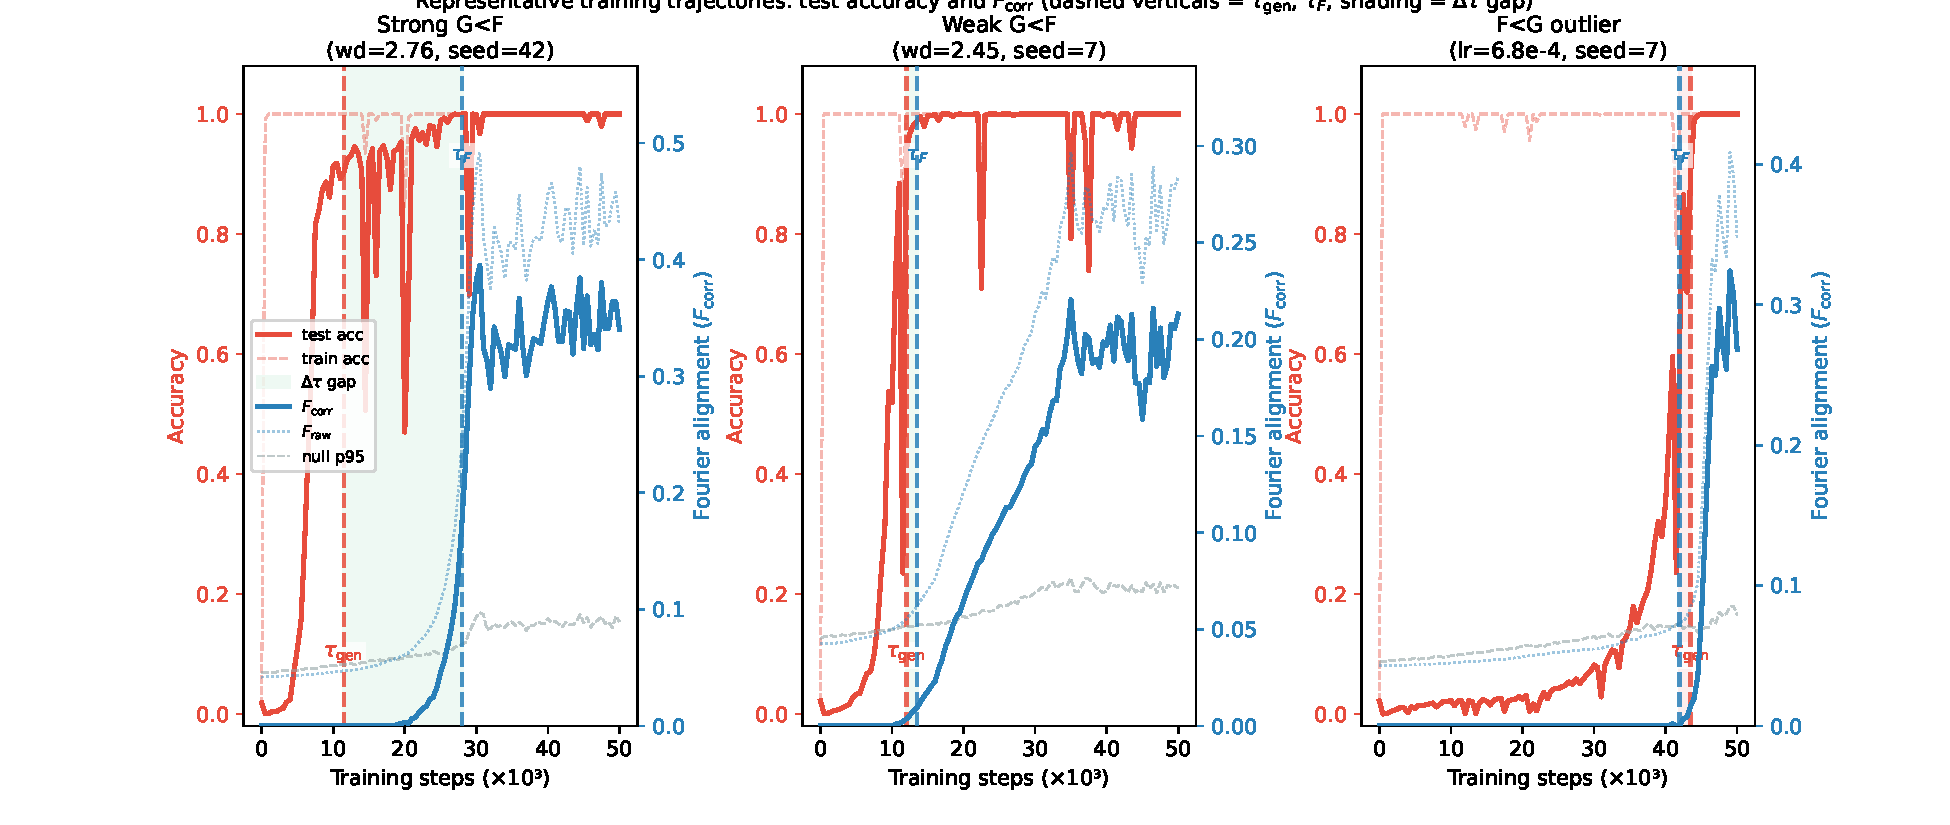
\includegraphics[width=0.85\textwidth]{timeline_example.pdf}
  \caption{Representative single-run timeline. Top: test accuracy
    with the $\taug$ threshold crossing marked. Bottom: null-corrected
    Fourier alignment $\fcorr(t)$ with the BIC-selected changepoint
    $\tauf$ marked. The signed lag $\Dtau = \tauf - \taug$ is the
    primary outcome variable of this project.}
  \label{fig:timeline_example}
\end{figure}

\textbf{Stage~0 (Metric Validation).}
Six representative cells (two each from expected Grokking,
Memorisation, and Confusion regions) will be run with 3 seeds each
to validate that $\taug$ and $\tauf$ behave as expected and to
confirm that the chosen metric thresholds are appropriate before
committing to full-scale sweeps.

\textbf{Stage~1 (Coarse Grid).}
A 5$\times$5 grid spanning the ($\mathrm{lr}$, $\mathrm{wd}$)
hyperparameter space will be run with 1 seed per cell to map phase
boundaries and identify G$<$F signal.

\textbf{Stage~2 (Weight Decay Sweep).}
Fixed $\mathrm{lr} = 1.6\times10^{-3}$: this value sits near the centre
of the Grokking band identified in the Stage~1 coarse grid---it
produced the clearest generalisation transitions across the widest
range of weight decays, so holding lr fixed here isolates the
wd-dependent structure of $\Dtau$.
Weight decay: 10 log-spaced values in $[1.2, 3.5]$:
$\{1.20, 1.35, 1.52, 1.71, 1.93, 2.18, 2.45, 2.76, 3.11, 3.50\}$.
The range is chosen to bracket the Stage~1 Grokking--Memorisation
boundary on both sides while staying inside the Grokking phase at
its centre.
Seeds $\{42, 7, 2025\}$. Total: 30 runs.

\textbf{Stage~3 (Learning Rate Sweep).}
Fixed $\mathrm{wd} = 2.5$: this is the median of the wd values at
which Stage~1 robustly produced Grokking, and it lies near the
centre of the wd plateau characterised in Stage~2, making it the
natural choice for isolating the lr-dependent structure of $\Dtau$.
Learning rate: 10 log-spaced values in $[5\times10^{-4}, 8\times10^{-3}]$:
$\{5.0, 6.8, 9.3, 12.6, 17.1, 23.3, 31.7, 43.2, 58.8, 80.0\}
\times 10^{-4}$.
The range extends roughly half a decade on either side of the
Stage~2 centre ($\mathrm{lr} = 1.6\times10^{-3}$) to probe both the
slow-learning and fast-learning edges of the Grokking phase.
Seeds $\{42, 7, 2025\}$. Total: 30 runs.

\textbf{Sensitivity Analysis.}
To reduce ad hoc cell selection, the subset of cells re-analysed
under alternative detector settings is determined by a fixed
secondary-analysis rule applied to the initial Stage~2$+$Stage~3
classification table (i.e., the rule itself is specified once and
then applied mechanically, rather than chosen cell-by-cell after
inspecting each run):
(i)~stratified sampling of the Grokking-phase cells into quintiles of
$|\Dtau|$ and selection of the median cell from each quintile
(5 cells);
(ii)~all cells classified as coincident ($|\Dtau|\leq 500$~steps);
(iii)~all cells classified as F$<$G, if any;
(iv)~3 cells classified as Memorisation and 3 as F\_only, as
negative controls.
Each selected cell is then re-analysed under all
$3\times4\times3 = 36$ detector configurations, varying the
null-update interval $\{2{,}500, 5{,}000, 10{,}000\}$, the EMA
smoothing coefficient $\alpha\in\{0.05, 0.10, 0.15, 0.25\}$, and
the BIC slope threshold $\{0.5\%, 1\%, 2\%\}$.

\section{Expected Outcomes}

If the G$<$F hypothesis holds, we expect:
\begin{itemize}
  \item The majority of Grokking-phase runs will show positive $\Dtau$
    (generalisation precedes Fourier embedding alignment), with a
    consistent margin of several thousand training steps.
  \item The G$<$F pattern will persist across both the weight-decay axis
    (Stage~2) and the learning-rate axis (Stage~3), indicating it is a
    property of the Grokking phase rather than an artefact of a single
    hyperparameter setting.
  \item The finding will be robust to detector hyperparameter choices:
    varying the null-update interval, EMA smoothing coefficient, and BIC
    slope threshold should not reverse the ordering for runs with large
    $|\Dtau|$.
\end{itemize}

If F$<$G holds instead, or if the ordering is inconsistent across the
phase diagram, this would suggest that embedding-level Fourier structure
is a prerequisite for generalisation rather than a lagging consolidation
step---a qualitatively different picture of the grokking process.

A secondary expected outcome is a characterisation of \textbf{F\_only}
runs (Fourier geometry detected without generalisation), which would
illuminate whether embedding alignment is necessary, sufficient, or
neither for generalisation.

\section{Anticipated Limitations}

\begin{itemize}
  \item \textbf{Single task}: experiments are restricted to
    $(a+b)\bmod 53$; the generality of the G$<$F finding to other
    modular or non-modular tasks remains an open question.
  \item \textbf{1D confirmatory sweeps}: after the initial coarse 2D
    grid (Stage~1), each confirmatory stage fixes one hyperparameter
    axis; a dense 2D grid over both axes simultaneously would provide
    stronger coverage of the full Grokking region.
  \item \textbf{Resolution floor}: $\Dtau$ is measured at 500-step
    intervals; small lags ($|\Dtau|\lesssim500$ steps) cannot be
    reliably classified as one ordering or the other.
  \item \textbf{Circuit formation not measured}: this project measures
    the timing gap between generalisation onset and embedding-geometry
    onset; the earlier circuit-formation stage is not directly tracked
    in the same runs.
\end{itemize}

\section{Risk Assessment}

\subsection{OHS Risk Assessment}

This project is entirely computational: all work involves writing
and running Python code on a personal workstation, with long-running
sweeps occasionally off-loaded to rented cloud GPU instances (RTX PRO
6000, A800) accessed remotely via SSH.
No laboratory, field, or wet-lab work of any kind is involved; no
hazardous materials, chemicals, biological agents, high-voltage
equipment, or physical prototypes are handled; and the cloud GPU
hardware is owned and physically maintained by the data-centre
provider with no physical access required of the researcher.
The project therefore falls under the \textbf{Low Risk} category and
is covered by the general OHS laboratory rules of the School of EECS.
The primary ergonomic considerations (prolonged computer use) will be
managed by taking regular breaks in accordance with standard university
guidance.

\subsection{Ethics Assessment}

This project does not involve human participants, animal subjects,
or the collection of personal data.
All experiments are conducted on synthetically generated arithmetic
datasets ($\{(a,b,c) \mid a+b \equiv c \pmod{53}\}$) with no
identifiable individuals.
No UQ ethical clearance is required.

\subsection{Project Schedule Risks}

\begin{itemize}
  \item \textbf{Computational runtime}: each full sweep (30 runs
    $\times$ 50{,}000--80{,}000 steps) may exceed initial time
    estimates if convergence is slow.
    \textit{Mitigation}: runs are primarily parallelised on a local
    GPU (RTX 4080) with longer-running sweeps off-loaded to rented
    cloud GPUs (RTX PRO 6000, A800) as needed;
    if time is insufficient, sweep resolution can be reduced without
    compromising the primary research question.
  \item \textbf{Hardware failure}: GPU malfunction could interrupt
    experiments.
    \textit{Mitigation}: checkpoints are saved every 500 steps; runs
    can be resumed or migrated to a cloud GPU instance.
  \item \textbf{Detector non-detection}: $\tauf$ may not be detected
    in a substantial fraction of runs, reducing sample size for the
    ordering analysis.
    \textit{Mitigation}: the F\_only label already accounts for this
    case; $\taug$ alone constitutes a valid secondary contribution.
  \item \textbf{Scope creep}: the sensitivity analysis (36 configurations)
    is the most time-intensive optional component.
    \textit{Mitigation}: it is scheduled last (Weeks 9--10) and can
    be scoped down to fewer configurations if needed.
\end{itemize}

\section{Project Milestones and Timeline}
\label{sec:milestones}

\begin{table}[htbp]
  \centering
  \caption{Project milestones, resources, planned timeline, and current status.}
  \label{tab:milestones}
  \renewcommand{\arraystretch}{1.2}
  \setlength{\tabcolsep}{4pt}
  \small
  \begin{tabular}{p{2.1cm}p{4.6cm}p{3.2cm}p{1.7cm}p{1.5cm}}
    \toprule
    Milestone & Description & Resources & Planned Weeks & Status \\
    \midrule
    Stage~0 & Metric validation (6 cells $\times$ 3 seeds) & $\sim$6~GPU-h, $<$1~GB disk & Weeks 1--2 & Complete \\
    Stage~1 & Coarse 5$\times$5 grid sweep (25 runs) & $\sim$12~GPU-h, $\sim$2~GB disk & Weeks 3--4 & Complete \\
    Stage~2 & Weight-decay axis sweep (30 runs) & $\sim$15~GPU-h, $\sim$2~GB disk & Weeks 5--6 & Complete \\
    Stage~3 & Learning-rate axis sweep (30 runs) & $\sim$15~GPU-h, $\sim$2~GB disk & Weeks 7--8 & Complete \\
    Sensitivity & 36-configuration detector robustness analysis (post-hoc on saved checkpoints) & $\sim$4~CPU-h, negligible disk & Weeks 9--10 & Complete \\
    Write-up (draft) & Chapters 1--3 first draft; figures integrated & Writing only & Week 11 & In progress \\
    Write-up (revision) & Supervisor review, incorporate feedback & Writing only & Week 12 & Pending \\
    Write-up (submit) & Final proof-read and submission & Writing only & Week 13 & Pending \\
    \bottomrule
  \end{tabular}
\end{table}

As of the time of submission, Stages~0 through~3 and the sensitivity
analysis have been completed on schedule.
Experiment data and analysis scripts are archived under
\texttt{runs/}, \texttt{src/}, and \texttt{notebooks/} in the project
repository.
The remaining deliverable is the final thesis write-up
(Weeks~11--13), which is currently in progress.
The majority of experiments were run on a local GPU workstation
(NVIDIA RTX 4080 Laptop, 12~GB VRAM); a smaller subset of
longer-running sweeps was executed on rented cloud GPU instances
(NVIDIA RTX PRO 6000 and NVIDIA A800).
The software stack is Python~3.14, PyTorch~2.5, and CUDA~12.4.

{\renewcommand{\bibname}{References}%
\begin{thebibliography}{99}
\addcontentsline{toc}{chapter}{References}

\bibitem{anthropic2024claudecode}
Anthropic, ``Claude Code,'' AI coding assistant (Claude Sonnet
family of models), 2024--2026.
[Online]. Available: \url{https://www.anthropic.com/claude-code}
(Accessed: Apr.~21, 2026).

\bibitem{openai2024chatgpt}
OpenAI, ``ChatGPT (GPT-5.4),'' large language model, 2026.
[Online]. Available: \url{https://chat.openai.com}
(Accessed: Apr.~21, 2026).

\bibitem{power2022grokking}
A.~Power, Y.~Burda, H.~Edwards, I.~Babuschkin, and V.~Misra,
``Grokking: Generalization Beyond Overfitting on Small Algorithmic
Datasets,'' \textit{arXiv preprint arXiv:2201.02177}, 2022.

\bibitem{nanda2023progress}
N.~Nanda, L.~Chan, T.~Lieberum, J.~Smith, and J.~Steinhardt,
``Progress Measures for Grokking via Mechanistic Interpretability,''
in \textit{International Conference on Learning Representations}, 2023.

\bibitem{liu2022towards}
Z.~Liu, O.~Kitouni, N.~Nolte, E.~J.~Michaud, M.~Tegmark, and
M.~Williams, ``Towards Understanding Grokking: An Effective Theory
of Representation Learning,'' in \textit{Advances in Neural
Information Processing Systems}, vol.~35, 2022.

\bibitem{liu2023omnigrok}
Z.~Liu, E.~J.~Michaud, and M.~Tegmark,
``Omnigrok: Grokking Beyond Algorithmic Data,''
in \textit{International Conference on Learning Representations},
2023.

\bibitem{thilak2022slingshot}
V.~Thilak, E.~Littwin, S.~Zhai, O.~Saremi, R.~Paiss, and J.~Susskind,
``The Slingshot Mechanism: An Empirical Study of Adaptive Optimizers
and the Grokking Phenomenon,''
\textit{arXiv preprint arXiv:2206.04817}, 2022.

\bibitem{doshi2024grok}
D.~Doshi, A.~Das, T.~He, and A.~Gromov,
``To Grok or not to Grok: Disentangling Generalization and Memorization
on Corrupted Algorithmic Datasets,''
in \textit{International Conference on Learning Representations}, 2024.

\bibitem{gromov2023grokking}
A.~Gromov,
``Grokking Modular Arithmetic,''
\textit{arXiv preprint arXiv:2301.02679}, 2023.

\bibitem{zhong2023clock}
Z.~Zhong, Z.~Liu, M.~Tegmark, and J.~Andreas,
``The Clock and the Pizza: Two Stories in Mechanistic Explanation
of Neural Networks,''
in \textit{Advances in Neural Information Processing Systems}, 2023.

\bibitem{chughtai2023toy}
B.~Chughtai, L.~Chan, and N.~Nanda,
``A Toy Model of Universality: Reverse Engineering How Networks
Learn Group Operations,''
in \textit{International Conference on Machine Learning}, 2023.

\bibitem{varma2023explaining}
V.~Varma, R.~Shah, Z.~Kenton, J.~Kram{\'a}r, and R.~Kumar,
``Explaining Grokking Through Circuit Efficiency,''
\textit{arXiv preprint arXiv:2309.02390}, 2023.

\bibitem{barak2022hidden}
B.~Barak, B.~L.~Edelman, S.~Goel, S.~Kakade, E.~Malach, and
C.~Zhang, ``Hidden Progress in Deep Learning: SGD Learns Parities
Near the Computational Limit,'' in \textit{Advances in Neural
Information Processing Systems}, vol.~35, 2022.

\bibitem{saxe2014exact}
A.~M.~Saxe, J.~L.~McClelland, and S.~Ganguli,
``Exact Solutions to the Nonlinear Dynamics of Learning in Deep
Linear Neural Networks,''
in \textit{International Conference on Learning Representations}, 2014.

\bibitem{elhage2021mathematical}
N.~Elhage, N.~Nanda, C.~Olsson, T.~Henighan, N.~Joseph, B.~Mann,
et~al., ``A Mathematical Framework for Transformer Circuits,''
Anthropic, \textit{Transformer Circuits Thread}, web publication,
Dec.~2021.
[Online]. Available:
\url{https://transformer-circuits.pub/2021/framework/index.html}
(Accessed: Apr.~21, 2026).

\bibitem{rubin2024grokking}
N.~Rubin, I.~Seroussi, and Z.~Ringel,
``Grokking as a First Order Phase Transition in Two Layer Networks,''
in \textit{International Conference on Learning Representations}, 2024.

\bibitem{kumar2024lazy}
T.~Kumar, B.~Bordelon, S.~J.~Gershman, and C.~Pehlevan,
``Grokking as the Transition from Lazy to Rich Training Dynamics,''
in \textit{International Conference on Learning Representations}, 2024.

\bibitem{lyu2024dichotomy}
K.~Lyu, J.~Jin, Z.~Li, S.~S.~Du, J.~D.~Lee, and W.~Hu,
``Dichotomy of Early and Late Phase Implicit Biases Can Provably
Induce Grokking,''
in \textit{International Conference on Learning Representations}, 2024.

\bibitem{mohamadi2024grok}
M.~A.~Mohamadi, Z.~Li, L.~Wu, and D.~J.~Sutherland,
``Why Do You Grok? A Theoretical Analysis on Grokking Modular
Addition,''
in \textit{International Conference on Machine Learning}, 2024.

\bibitem{vaswani2017attention}
A.~Vaswani, N.~Shazeer, N.~Parmar, J.~Uszkoreit, L.~Jones,
A.~N.~Gomez, {\L}.~Kaiser, and I.~Polosukhin,
``Attention Is All You Need,''
in \textit{Advances in Neural Information Processing Systems},
vol.~30, 2017.

\bibitem{loshchilov2019decoupled}
I.~Loshchilov and F.~Hutter,
``Decoupled Weight Decay Regularization,''
in \textit{International Conference on Learning Representations}, 2019.

\bibitem{schwarz1978estimating}
G.~Schwarz,
``Estimating the Dimension of a Model,''
\textit{The Annals of Statistics}, vol.~6, no.~2, pp.~461--464, 1978.

\end{thebibliography}

\end{document}
